\chapter{Proposta do trabalho}

Conforme descrito no Capítulo \ref{cap:introducao}, este trabalho será constituído de cinco etapas.
Em um primeiro momento, a etapa de diagnóstico foi realizada e os sistemas relacionados e suas funcionalidades em comum 
foram apresentadas no Capítulo \ref{cap:sistemas_relacionados}. Neste capítulo é apresentado o resultado da segunda etapa
que é a descrição da proposta do trabalho de acordo com os objetivos estabelecidos.

Para a plataforma Empurrando Juntos é prevista uma arquitetura cliente-servidor a fim de possibilitar a criação de aplicações e
aplicativos. A estrutura que contempla o lado servidor é denominada Pentano e pode ser visualizada na Figura \ref{fig:pentano}. 
O Pentano é constituído por dois módulos: o \textit{server}, 
que é o módulo da API a ser criada neste trabalho e o \textit{Math} que é o módulo responsável pela clusterização. 

\begin{figure}[h!]
\centering
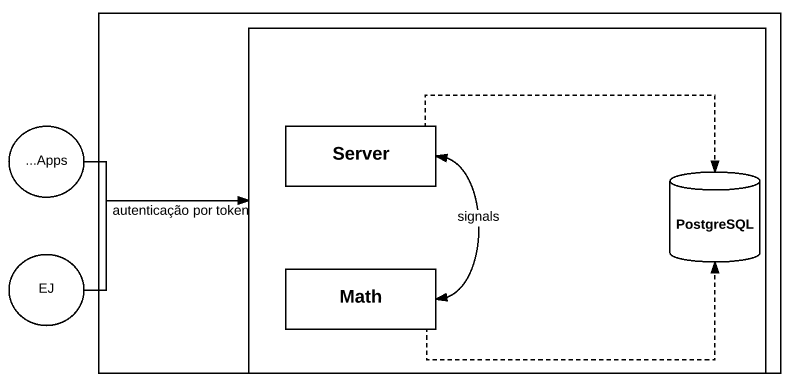
\includegraphics[scale=0.8]{figuras/esquema_pentano.png}
\caption{Estrutura do Pentano}
\label{fig:pentano}
\end{figure}

\section{Requisitos da solução}

Uma avaliação do escopo da plataforma Empurrando Juntos permitiu o levantamento de características do sistema e por consequência
os requisitos associados, o que foi resumido na Tabela \ref{tab:requisitos}.

\begin{table}[h!]
\centering
\caption{Requisitos da aplicação}
\label{tab:requisitos}
\begin{tabular}{@{}cl@{}}
\toprule
\textbf{Característica}                      & \multicolumn{1}{c}{\textbf{Requisito}}                                                                                                \\ \midrule
\multirow{4}{*}{Gerenciamento de Usuário}    & O sistema deve permitir o cadastro de usuários                                                                                        \\
                                             & O sistema deve permitir a alteração de usuários                                                                                       \\
                                             & O sistema deve permitir a exclusão de usuários                                                                                         \\
                                             & O sistema deve permitir login pelo facebook                                                                                           \\\midrule
\multirow{3}{*}{Gerenciamento de Conversa}   & O sistema deve permitir o cadastro de conversas                                                                                       \\
                                             & O sistema deve permitir a alteração de conversas                                                                                      \\
                                             & O sistema deve permitir a exclusão de conversas                                                                                       \\ \midrule
\multirow{4}{*}{Gerenciamento de Comentário} & O sistema deve permitir o cadastro de comentários em conversas                                                                        \\
                                             & O sistema deve permitir a alteração de comentários                                                                                    \\
                                             & O sistema deve permitir a exclusão de comentários                                                                                     \\ 
                                             & O sistema deve permitir que o usuário vote em comentários                                                                             \\ \midrule
Agrupamento de usuários                      & \begin{tabular}[c]{@{}l@{}}O sistema deve permitir a visualização dos usuários agrupados \\ de acordo com os votos dados\end{tabular} \\ \bottomrule
\end{tabular}
\end{table}


Para contemplar os requisitos elicitados foram mapeadas as entidades principais, alguns de seus atributos e os relacionamentos entre elas. 
Esse mapeamento pode ser visto na Figura \ref{fig:entidades}.

\begin{figure}[h!]
\centering
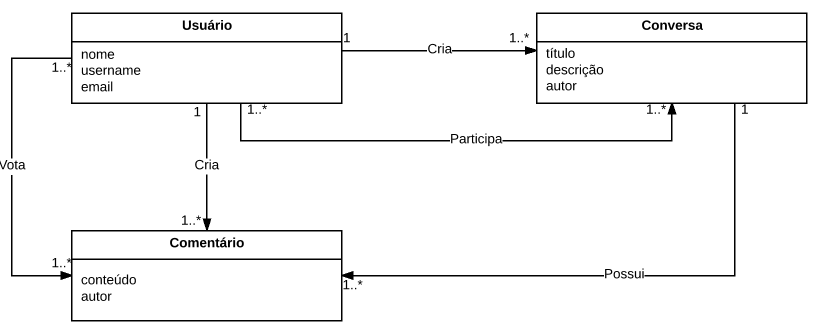
\includegraphics[scale=0.6]{figuras/entidades.png}
\caption{Entidades da API}
\label{fig:entidades}
\end{figure}

Os requisitos supracitados e as entidades mapeadas serão providas para a plataforma por meio dos serviços REST a serem implementados.
A tecnologia escolhida para implementação da API foi a linguagem Python juntamente com os \textit{frameworks} Django e Django Rest Framework.

Considerando a estrutura proposta pelo Empurrando Juntos e a tecnologia escolhida foram identificados os seguintes requisitos não funcionais:

\begin{itemize}
 \item Autenticação por token;
 \item Definição dinâmica da semântica dos votos;
 \item Integração com o módulo \textit{Math};
 \item Utilização do PEP8.
\end{itemize}


% Para execução do trabalho foi estabelecido um cronograma que pode ser visto na Figura \ref{fig:cronograma}.
% Foram contempladas as atividades iniciais realizadas e o planejamento para implementação da solução.
% O desenvolvimento da API será por meio de um processo iterativo e incremental. 

% \begin{figure}[h!]
% \centering
% 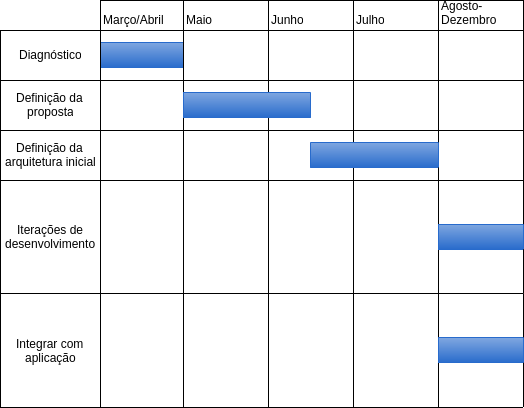
\includegraphics[scale=0.6]{figuras/cronograma.png}
% \caption{Cronograma de execução}
% \label{fig:cronograma}
% \end{figure}

% \section{Resultados Esperados}

% No final do trabalho é esperado uma API Rest que seja capaz de fornecer um serviço de participação com conversas, comentários
% e votos que agrupe pessoas de acordo com os votos.

% Com esse serviço, espera-se contribuir com a plataforma Empurrando Juntos através da implementação da parte servidor da 
% arquitetura definida.

% Dentro do contexto social, o objetivo é que a API possa contribuir no apoio à mulheres vítimas de violência, através
% da promoção de discussões mais efetivas e a criação de uma rede de apoio entre mulheres que passam ou passaram por essa situação.








